%************************************************
\chapter{Purification by Sublimation}
%************************************************
\begin{flushright}
April 15, 2013
\end{flushright}
\section{Aim}
To demonstrate the sublimation of Napthalene as a viable method of purification

\section {Chemicals Required}
	\begin{enumerate}
		\item Naphthalene
	\end{enumerate}

\section{Theory}
	There are three typical states of matter, viz. Solid, Liquid and gas. There can be more states depending on the specific system in question.
	\par
	\emph{Sublimation} is the transition of a substance from the solid phase to its gaseous phase without transitioning through the liquid phase.
	\par
	Sublimation is an \emph{endothermic} phase transition that occurs at temperatures and pressures below the triple point of the material being studied.
	\par
	For high triple points, the change in temperature and/or pressure results in the disturbance of the solid-vapour phase equilibrium. Refer to the phase diagram given in \autoref{e12_phase}
	\par
	For Naphthalene, the atmospheric pressure is below its triple point \footnote{For Naphthalene we have,
	\begin{align*}
		\text{Molecular Formula} &= C_{10}H_8 \\
		\text{Triple Point} &= 0.99 kPa \\
		\text{Triple Point Temperature} &= 353.3 K = 80.15 ^o C
	\end{align*}	
	}. Thus when it is heated in an open vessel, the phase changes directly to the vapour phase, as expected.
	\par
	Substances that do not sublime at atmospheric pressure may also be purified by this technique by lowering the pressure.
	\par
	The idea is that the impurities would not sublime and the substance desired would.
	
	\begin{figure}[bth]
		\begin{center}
			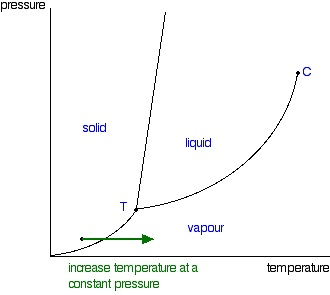
\includegraphics[width=1.0\linewidth]{gfx/e12_phase}
		\end{center}
	\caption[Phase Diagram]{Phase Diagram} {\label{e12_phase}}
	\end{figure}


\section{Experimental Setup}
	Naphthalene was taken in a china dish. An inverted funnel was placed over it and cotton was used to block the opening. This was heated from the bottom and over a period of time, white spots could be observed on the inner surface of the funnel.

\section{Acknowledgements}
I thank our PhD guide for demonstrating the experiment, and also the lab assistants, including Mr. Mangat.
\par
\url{http://www.chemeo.com/} was referred to for the data on Naphthalene.
\par
The sublimation phase diagram was taken from \url{http://chemguide.co.uk}